\documentclass{beamer}
\usetheme{AnnArbor}
\usecolortheme{spruce}
\usepackage{circuitikz}
\usepackage{graphicx}
\usepackage{verbatim}

\title{Sequential Programming, Latches, Flip-Flops}
\subtitle{(Not the beach footwear)}
\author[CMSC389E]{Akilesh Praveen | CMSC398E}
\institute{UMD}
\date{\today}

\begin{document}

    % title page
    \begin{frame}
        \titlepage
    \end{frame}
    
    % table of contents
    \begin{frame}
        \frametitle{Agenda}
        \tableofcontents
    \end{frame}
    
    \section{Announcements}
    
        \begin{frame}
                \vfill
                \centering
                \begin{beamercolorbox}[sep=8pt,center,shadow=true,rounded=true]{title}
                    \usebeamerfont{title}Announcements\par%
                \end{beamercolorbox}
                \vfill
             \end{frame}
    
        \subsection{Online Classes}
        
            
            
            \begin{frame}
                \frametitle{Online Classes!}
                \begin{itemize}
                    \item Class will be online for the \textbf{rest of spring 2020}.
                    \item What does this mean for us?
                    \item Lecture will now be held at \textbf{2PM EST} on \textbf{Discord}. If you cannot make it, lecture will be recorded and uploaded to an accessible location (TBA on Piazza).
                    \item The CS Submit server is open for business!
                    
                \end{itemize}
            \end{frame}
            
        \subsection{Online Resources}
            
            \begin{frame}
            	\frametitle{Online Resources}
            	\begin{itemize}
            		\item Here's a quick recap of all the resources that we've put together to help you learn and succeed in this class.
            		\begin{itemize}
            			\item \textbf{Piazza} is the place to ask questions and get answers. Ashwath will be posting frequently here about project and solution releases, so make sure to check in when you can.
            			\item \textbf{ELMS} is where you can take a look at your current grade in the class.
            			\item The \textbf{CS Submit Server} is where all your projects will be turned into. Ashwath's web app is how you'll accomplish this.
            			\item \textbf{The Course Website} is where you can find a cumulative guide for what we've covered in class, separated out by weeks. It's a much more organized way to see our weekly material than Piazza.
            			\item \textbf{Email} is the best and quickest way to reach your instructors.
            		\end{itemize}
            	\end{itemize}
            \end{frame}
            
            \begin{frame}
            	\frametitle{Discord}
            	\begin{itemize}
            		\item The Discord is up, and assuming that you are watching lecture right now, you've had no issue joining it. For those of you who are looking at this slideset and wish to join the discord, go ahead and check out the relevant ELMS announcement, where Ashwath has uploaded the invite link.
            		\item If you have any issues getting Discord set up, feel free to contact Ashwath or me for help.
            	\end{itemize}
            \end{frame}
			\subsection{Project Schedule and Guidelines}    
       
       		\begin{frame}
       			\frametitle{Project Schedule}
       			\begin{itemize}
       				\item Circumstances have led us to develop a new project schedule.
       			\end{itemize}
       		\end{frame}
       		
       		\begin{frame}
       			\frametitle{New Submission Guidelines}
       			\begin{itemize}
       				\item Now, you can submit your worldfiles to a web app, and testing should take place automatically on the CS submit server.
       				\item More information is available on Piazza, ELMS and Discord.
       			\end{itemize}
       		\end{frame}
        
    
   	\section{What is Sequential Logic?}
   	
   		\begin{frame}
   			\frametitle{What is Sequential Logic?}
   			\begin{itemize}
   				\item To understand sequential logic, first we have to make a note of what we know about \textbf{combinational logic}.
   				\item Combinational logic basically only relies on the initial inputs to make a decision.
   			\end{itemize}
   			
   			{
   			\centering
   			



\tikzset{every picture/.style={line width=0.75pt}} %set default line width to 0.75pt        

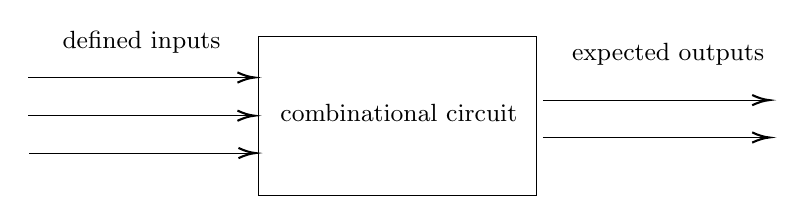
\begin{tikzpicture}[x=0.75pt,y=0.75pt,yscale=-.75,xscale=.75]
%uncomment if require: \path (0,300); %set diagram left start at 0, and has height of 300

%Shape: Rectangle [id:dp5841562830006607] 
\draw   (252,99.71) -- (431,99.71) -- (431,202) -- (252,202) -- cycle ;
%Straight Lines [id:da44338869137483317] 
\draw    (104.33,126.33) -- (247.67,126.33) ;
\draw [shift={(249.67,126.33)}, rotate = 180] [color={rgb, 255:red, 0; green, 0; blue, 0 }  ][line width=0.75]    (10.93,-3.29) .. controls (6.95,-1.4) and (3.31,-0.3) .. (0,0) .. controls (3.31,0.3) and (6.95,1.4) .. (10.93,3.29)   ;
%Straight Lines [id:da114016208212253] 
\draw    (104.33,150.86) -- (247.67,150.86) ;
\draw [shift={(249.67,150.86)}, rotate = 180] [color={rgb, 255:red, 0; green, 0; blue, 0 }  ][line width=0.75]    (10.93,-3.29) .. controls (6.95,-1.4) and (3.31,-0.3) .. (0,0) .. controls (3.31,0.3) and (6.95,1.4) .. (10.93,3.29)   ;
%Straight Lines [id:da8667122570412495] 
\draw    (105,174.86) -- (248.33,174.86) ;
\draw [shift={(250.33,174.86)}, rotate = 180] [color={rgb, 255:red, 0; green, 0; blue, 0 }  ][line width=0.75]    (10.93,-3.29) .. controls (6.95,-1.4) and (3.31,-0.3) .. (0,0) .. controls (3.31,0.3) and (6.95,1.4) .. (10.93,3.29)   ;
%Straight Lines [id:da8048516099848341] 
\draw    (435,164.86) -- (578.33,164.86) ;
\draw [shift={(580.33,164.86)}, rotate = 180] [color={rgb, 255:red, 0; green, 0; blue, 0 }  ][line width=0.75]    (10.93,-3.29) .. controls (6.95,-1.4) and (3.31,-0.3) .. (0,0) .. controls (3.31,0.3) and (6.95,1.4) .. (10.93,3.29)   ;
%Straight Lines [id:da5461614070052315] 
\draw    (435,140.86) -- (578.33,140.86) ;
\draw [shift={(580.33,140.86)}, rotate = 180] [color={rgb, 255:red, 0; green, 0; blue, 0 }  ][line width=0.75]    (10.93,-3.29) .. controls (6.95,-1.4) and (3.31,-0.3) .. (0,0) .. controls (3.31,0.3) and (6.95,1.4) .. (10.93,3.29)   ;

% Text Node
\draw (124.67,94.67) node [anchor=north west][inner sep=0.75pt]   [align=left] {{\small defined inputs}};
% Text Node
\draw (452,102.67) node [anchor=north west][inner sep=0.75pt]   [align=left] {{\small expected outputs}};
% Text Node
\draw (264.67,142) node [anchor=north west][inner sep=0.75pt]   [align=left] {{\small combinational circuit}};


\end{tikzpicture}


   			
   			}
   			
   			\begin{itemize}
   				\item In other words, we've had a \textbf{set truth table} for our combinational circuits; knowing the inputs means you know the outputs.
   				\item \textit{"Your next line will be... "}
   			\end{itemize}
   		\end{frame}
   		
   		
   		\subsection{Sequential Logic}
   		
   		\begin{frame}
                \vfill
                \centering
                \begin{beamercolorbox}[sep=8pt,center,shadow=true,rounded=true]{title}
                    \usebeamerfont{title}Sequential Logic\par%
                \end{beamercolorbox}
                \vfill
             \end{frame}
   		
   		\begin{frame}
   			\frametitle{What is Sequential Logic?}
   			\begin{itemize}
   				\item When it comes to sequential logic, the whole point is \textbf{not knowing in one cycle what your output is}.
   				\item In other words, these circuits don't just use the initial inputs, they use the outputs of previous iterations of the circuit to decide the output.
   			\end{itemize}
   			
   			{\centering
   			
   			

\tikzset{every picture/.style={line width=0.75pt}} %set default line width to 0.75pt        

\begin{tikzpicture}[x=0.75pt,y=0.75pt,yscale=-1,xscale=1]
%uncomment if require: \path (0,300); %set diagram left start at 0, and has height of 300

%Shape: Rectangle [id:dp5841562830006607] 
\draw   (241.7,89.71) -- (345.99,89.71) -- (345.99,188.67) -- (241.7,188.67) -- cycle ;
%Straight Lines [id:da44338869137483317] 
\draw    (155.67,115.47) -- (238.34,115.47) ;
\draw [shift={(240.34,115.47)}, rotate = 180] [color={rgb, 255:red, 0; green, 0; blue, 0 }  ][line width=0.75]    (10.93,-3.29) .. controls (6.95,-1.4) and (3.31,-0.3) .. (0,0) .. controls (3.31,0.3) and (6.95,1.4) .. (10.93,3.29)   ;
%Straight Lines [id:da114016208212253] 
\draw    (155.67,139.19) -- (238.34,139.19) ;
\draw [shift={(240.34,139.19)}, rotate = 180] [color={rgb, 255:red, 0; green, 0; blue, 0 }  ][line width=0.75]    (10.93,-3.29) .. controls (6.95,-1.4) and (3.31,-0.3) .. (0,0) .. controls (3.31,0.3) and (6.95,1.4) .. (10.93,3.29)   ;
%Straight Lines [id:da8667122570412495] 
\draw    (156.06,162.41) -- (238.73,162.41) ;
\draw [shift={(240.73,162.41)}, rotate = 180] [color={rgb, 255:red, 0; green, 0; blue, 0 }  ][line width=0.75]    (10.93,-3.29) .. controls (6.95,-1.4) and (3.31,-0.3) .. (0,0) .. controls (3.31,0.3) and (6.95,1.4) .. (10.93,3.29)   ;
%Straight Lines [id:da8048516099848341] 
\draw    (348.32,152.73) -- (431,152.73) ;
\draw [shift={(433,152.73)}, rotate = 180] [color={rgb, 255:red, 0; green, 0; blue, 0 }  ][line width=0.75]    (10.93,-3.29) .. controls (6.95,-1.4) and (3.31,-0.3) .. (0,0) .. controls (3.31,0.3) and (6.95,1.4) .. (10.93,3.29)   ;
%Straight Lines [id:da5461614070052315] 
\draw    (348.32,129.52) -- (431,129.52) ;
\draw [shift={(433,129.52)}, rotate = 180] [color={rgb, 255:red, 0; green, 0; blue, 0 }  ][line width=0.75]    (10.93,-3.29) .. controls (6.95,-1.4) and (3.31,-0.3) .. (0,0) .. controls (3.31,0.3) and (6.95,1.4) .. (10.93,3.29)   ;
%Curve Lines [id:da6673833672845702] 
\draw    (347,175.5) .. controls (526,207.5) and (81,207.5) .. (238,175.5) ;
\draw [shift={(238,175.5)}, rotate = 528.48] [color={rgb, 255:red, 0; green, 0; blue, 0 }  ][line width=0.75]    (10.93,-3.29) .. controls (6.95,-1.4) and (3.31,-0.3) .. (0,0) .. controls (3.31,0.3) and (6.95,1.4) .. (10.93,3.29)   ;
%Shape: Rectangle [id:dp7234006449913947] 
\draw  [fill={rgb, 255:red, 255; green, 255; blue, 255 }  ,fill opacity=1 ] (269.33,193.33) -- (325.67,193.33) -- (325.67,218.67) -- (269.33,218.67) -- cycle ;

% Text Node
\draw (276.33,195.33) node [anchor=north west][inner sep=0.75pt]   [align=left] {state};
% Text Node
\draw (132,130) node [anchor=north west][inner sep=0.75pt]   [align=left] {in};
% Text Node
\draw (438.67,130.67) node [anchor=north west][inner sep=0.75pt]   [align=left] {out};
% Text Node
\draw (277.33,131.67) node [anchor=north west][inner sep=0.75pt]   [align=left] {circuit};


\end{tikzpicture}

   			
   			}
   		\end{frame}
   		
   		\begin{frame}
   			\frametitle{How do we achieve this?}
   			\begin{itemize}
   				\item Actually, it turns out it isn't that bad.
   				\item We're just doing what the diagram says- feeding the outputs of our circuit back into our circuit for further processing!
   				\item If you want a programming analogy, think of a loop statement with a loop variable.
   				\item {
   			\centering
   				\verbatiminput{loop.py} %a
   			}
   			\end{itemize}
   		\end{frame}
   		
   		
   		\begin{frame}
   			\frametitle{Keeping Track of Values}
   			\begin{itemize}
   				\item Well, that Python segment may have made sense in our heads, but we're missing a key element to help us translate this into digital logic
   				\item We have no idea how to recurrently store the value of a variable every time our circuit executes
   				\item In other words, we're \textit{looping} back to the idea of memory!
   			\end{itemize}
   		\end{frame}
   		
   	
   	
   	\section{The Idea of 'Memory'}
   	
	\begin{frame}
                \vfill
                \centering
                \begin{beamercolorbox}[sep=8pt,center,shadow=true,rounded=true]{title}
                    \usebeamerfont{title}Memory: Latches\par%
                \end{beamercolorbox}
                \vfill
             \end{frame}   	
   	
   	
   		\begin{frame}
   			\frametitle{The First Ever 'Memory'}
   			\begin{itemize}
   				\item The first type of memory ever used was \textbf{chained 'not' gates}.
   				\item Go ahead and try to imagine what would happen to the output if the input was 1 or 0. Keep in mind that it's important to consider the output's state before this.
   			\end{itemize}

			{
			\centering
			
			

\tikzset{every picture/.style={line width=0.75pt}} %set default line width to 0.75pt        

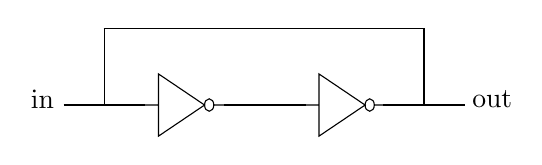
\begin{tikzpicture}[x=0.75pt,y=0.75pt,yscale=-1,xscale=1]
%uncomment if require: \path (0,300); %set diagram left start at 0, and has height of 300

%Straight Lines [id:da4397257544472163] 
\draw    (151,179) -- (190.33,179) ;
%Shape: Not/Inverter Gate [id:dp25857728507845545] 
\draw   (196.74,164) -- (218.96,179) -- (196.74,194) -- (196.74,164) -- cycle (189.33,179) -- (196.74,179) (223.41,179) -- (229.33,179) (218.96,179) .. controls (218.96,177.34) and (219.96,176) .. (221.19,176) .. controls (222.41,176) and (223.41,177.34) .. (223.41,179) .. controls (223.41,180.66) and (222.41,182) .. (221.19,182) .. controls (219.96,182) and (218.96,180.66) .. (218.96,179) -- cycle ;
%Straight Lines [id:da762390149891069] 
\draw    (228.33,179) -- (267.67,179) ;
%Shape: Not/Inverter Gate [id:dp46101602884334025] 
\draw   (274.07,164) -- (296.3,179) -- (274.07,194) -- (274.07,164) -- cycle (266.67,179) -- (274.07,179) (300.74,179) -- (306.67,179) (296.3,179) .. controls (296.3,177.34) and (297.29,176) .. (298.52,176) .. controls (299.75,176) and (300.74,177.34) .. (300.74,179) .. controls (300.74,180.66) and (299.75,182) .. (298.52,182) .. controls (297.29,182) and (296.3,180.66) .. (296.3,179) -- cycle ;
%Straight Lines [id:da2252257910210872] 
\draw    (305,179) -- (344.33,179) ;
%Straight Lines [id:da21519615454198027] 
\draw    (170.67,142) -- (170.67,179) ;
%Straight Lines [id:da7799654938921396] 
\draw    (324.67,142) -- (324.67,179) ;
%Straight Lines [id:da8861099279045884] 
\draw    (170.33,142) -- (324.67,142) ;

% Text Node
\draw (134,170.5) node [anchor=north west][inner sep=0.75pt]   [align=left] {in};
% Text Node
\draw (346.67,170.5) node [anchor=north west][inner sep=0.75pt]   [align=left] {out};


\end{tikzpicture}

			
			}   			
   			
   			\begin{itemize}
   				\item You'll find that the output stays at 0 until the input becomes a 1. Then, no matter what the input changes back to, the output will still stay at one.
   				\item This keeps track of \textit{something}, but since we can really only set it once, this probably isn't going to help us much in the long run.
   			\end{itemize}
   		\end{frame}
   		
   	
   	\section{Latches}
   	
   		\begin{frame}
   			\frametitle{Latches}
   			\begin{itemize}
   				\item We want to do more than set the value of memory just once.
   				\item You could also say that we want to be able to \textbf{reset} it.
   				\item I invite you to think for a moment- how can we augment the previous example to allow us to somehow 'reset' the state of our memory?
   				\item Unfortunately, it's not a one-off simple solution, so let's explore it together
   				
   			\end{itemize}
   		\end{frame}
   		
   		\begin{frame}
   			\frametitle{Latches}
   			\begin{itemize}
   				\item You can essentially perform this with a commonly-used circuit known as a latch
   				\item There are a few ways to build a latch, but we're going to look at the most basic latch today. (an \textbf{SR Latch})
   				\begin{itemize}
   					\item Specifically, a NOR SR Latch (made with NOR gates)
   				\end{itemize}
   				\item There are a few other latch designs that I'll be posting about under course resources. You can look at them on your own time, if you'd like.
   			\end{itemize}
   		\end{frame}
   		
   		\begin{frame}
   			\frametitle{NOR SR Latch}

			{
			\centering
			
			







\tikzset{every picture/.style={line width=0.75pt}} %set default line width to 0.75pt        

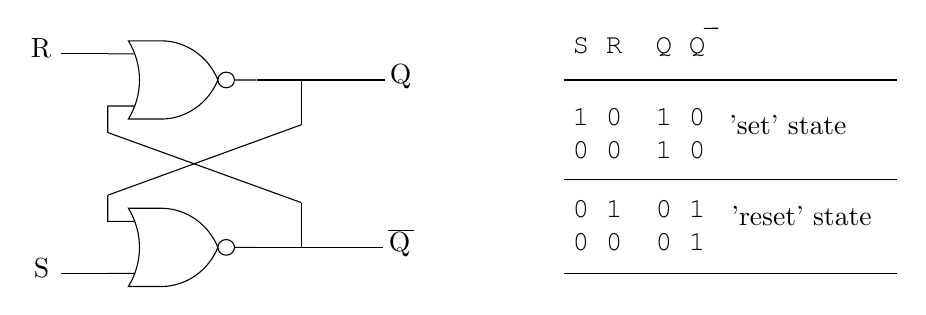
\begin{tikzpicture}[x=0.75pt,y=0.75pt,yscale=-1,xscale=1]
%uncomment if require: \path (0,300); %set diagram left start at 0, and has height of 300

%Shape: Nor Gate [id:dp4086281392337985] 
\draw   (106.27,101.83) -- (122.86,101.83) .. controls (134.43,102.17) and (144.77,109.51) .. (149.4,120.67) .. controls (144.77,131.82) and (134.43,139.16) .. (122.86,139.5) -- (106.27,139.5) .. controls (113.38,127.85) and (113.38,113.49) .. (106.27,101.83) -- cycle (96.31,108.11) -- (109.59,108.11) (96.31,133.22) -- (109.59,133.22) (157.36,120.67) -- (167.98,120.67) (149.4,120.67) .. controls (149.4,118.59) and (151.18,116.9) .. (153.38,116.9) .. controls (155.58,116.9) and (157.36,118.59) .. (157.36,120.67) .. controls (157.36,122.75) and (155.58,124.43) .. (153.38,124.43) .. controls (151.18,124.43) and (149.4,122.75) .. (149.4,120.67) -- cycle ;
%Shape: Nor Gate [id:dp06374716114881951] 
\draw   (106.27,182.5) -- (122.86,182.5) .. controls (134.43,182.84) and (144.77,190.18) .. (149.4,201.33) .. controls (144.77,212.49) and (134.43,219.83) .. (122.86,220.17) -- (106.27,220.17) .. controls (113.38,208.51) and (113.38,194.15) .. (106.27,182.5) -- cycle (96.31,188.78) -- (109.59,188.78) (96.31,213.89) -- (109.59,213.89) (157.36,201.33) -- (167.98,201.33) (149.4,201.33) .. controls (149.4,199.25) and (151.18,197.57) .. (153.38,197.57) .. controls (155.58,197.57) and (157.36,199.25) .. (157.36,201.33) .. controls (157.36,203.41) and (155.58,205.1) .. (153.38,205.1) .. controls (151.18,205.1) and (149.4,203.41) .. (149.4,201.33) -- cycle ;
%Straight Lines [id:da8971344370044351] 
\draw    (96.31,133.22) -- (96.33,146) ;
%Straight Lines [id:da013829413387980494] 
\draw    (96.3,176.22) -- (96.31,189) ;
%Straight Lines [id:da2426037289151266] 
\draw    (96.31,108.11) -- (74,108.11) ;
%Straight Lines [id:da7708764718452497] 
\draw    (96.31,213.89) -- (74,213.89) ;
%Straight Lines [id:da9929408811615777] 
\draw    (230,120.67) -- (168,120.67) ;
%Straight Lines [id:da9839096117813674] 
\draw    (229,201.33) -- (167,201.33) ;
%Straight Lines [id:da30996716656707235] 
\draw    (189.5,179.75) -- (96.33,146) ;
%Straight Lines [id:da6058158265884392] 
\draw    (189.5,179.72) -- (189.5,201.33) ;
%Straight Lines [id:da695661569482763] 
\draw    (189.5,120.67) -- (189.5,142.28) ;
%Straight Lines [id:da12170141018992597] 
\draw    (189.5,142.28) -- (96.3,176.22) ;
%Straight Lines [id:da04396196367938876] 
\draw    (231.5,193.33) -- (244,193.33) ;
%Straight Lines [id:da554306741226894] 
\draw    (316,120.67) -- (476.5,120.67) ;
%Straight Lines [id:da06237648747012303] 
\draw    (316,168.67) -- (476.5,168.67) ;
%Straight Lines [id:da0016632155121070191] 
\draw    (316,213.89) -- (476.5,213.89) ;
%Straight Lines [id:da7850418068934745] 
\draw    (383.5,95.83) -- (390.5,95.75) ;

% Text Node
\draw (231,112.11) node [anchor=north west][inner sep=0.75pt]   [align=left] {Q};
% Text Node
\draw (230.5,192.83) node [anchor=north west][inner sep=0.75pt]   [align=left] {Q};
% Text Node
\draw (58,99.61) node [anchor=north west][inner sep=0.75pt]   [align=left] {R};
% Text Node
\draw (59.5,205.33) node [anchor=north west][inner sep=0.75pt]   [align=left] {S};
% Text Node
\draw (319,133.17) node [anchor=north west][inner sep=0.75pt]   [align=left] {{\fontfamily{pcr}\selectfont 1 0 \ 1 0}\\{\fontfamily{pcr}\selectfont 0 0 \ 1 0 }};
% Text Node
\draw (319,98.67) node [anchor=north west][inner sep=0.75pt]   [align=left] {{\fontfamily{pcr}\selectfont S R \ Q Q}};
% Text Node
\draw (319,177.57) node [anchor=north west][inner sep=0.75pt]   [align=left] {{\fontfamily{pcr}\selectfont 0 1 \ 0 1}\\{\fontfamily{pcr}\selectfont 0 0 \ 0 1 }};
% Text Node
\draw (394.5,136.5) node [anchor=north west][inner sep=0.75pt]   [align=left] {'set' state};
% Text Node
\draw (395.5,180.33) node [anchor=north west][inner sep=0.75pt]   [align=left] {'reset' state};


\end{tikzpicture}







			}  			
   			
   			\begin{itemize}
   				\item This is basically a circuit that switches between two ouput states, depending on which of its two inputs has a signal coming through it
   				\item Here's the beauty of it- if there's no input coming in, its state remains unchanged
   			\end{itemize}
   		\end{frame}
   		
   		\begin{frame}
   			\frametitle{NOR SR Latch}

			{
			\centering
			
			







\tikzset{every picture/.style={line width=0.75pt}} %set default line width to 0.75pt        

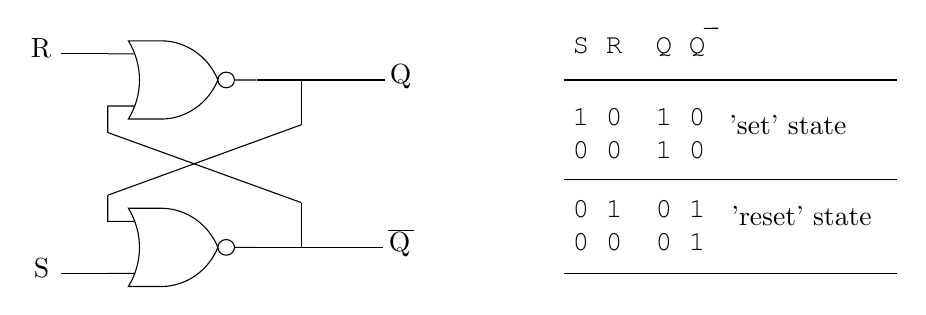
\begin{tikzpicture}[x=0.75pt,y=0.75pt,yscale=-1,xscale=1]
%uncomment if require: \path (0,300); %set diagram left start at 0, and has height of 300

%Shape: Nor Gate [id:dp4086281392337985] 
\draw   (106.27,101.83) -- (122.86,101.83) .. controls (134.43,102.17) and (144.77,109.51) .. (149.4,120.67) .. controls (144.77,131.82) and (134.43,139.16) .. (122.86,139.5) -- (106.27,139.5) .. controls (113.38,127.85) and (113.38,113.49) .. (106.27,101.83) -- cycle (96.31,108.11) -- (109.59,108.11) (96.31,133.22) -- (109.59,133.22) (157.36,120.67) -- (167.98,120.67) (149.4,120.67) .. controls (149.4,118.59) and (151.18,116.9) .. (153.38,116.9) .. controls (155.58,116.9) and (157.36,118.59) .. (157.36,120.67) .. controls (157.36,122.75) and (155.58,124.43) .. (153.38,124.43) .. controls (151.18,124.43) and (149.4,122.75) .. (149.4,120.67) -- cycle ;
%Shape: Nor Gate [id:dp06374716114881951] 
\draw   (106.27,182.5) -- (122.86,182.5) .. controls (134.43,182.84) and (144.77,190.18) .. (149.4,201.33) .. controls (144.77,212.49) and (134.43,219.83) .. (122.86,220.17) -- (106.27,220.17) .. controls (113.38,208.51) and (113.38,194.15) .. (106.27,182.5) -- cycle (96.31,188.78) -- (109.59,188.78) (96.31,213.89) -- (109.59,213.89) (157.36,201.33) -- (167.98,201.33) (149.4,201.33) .. controls (149.4,199.25) and (151.18,197.57) .. (153.38,197.57) .. controls (155.58,197.57) and (157.36,199.25) .. (157.36,201.33) .. controls (157.36,203.41) and (155.58,205.1) .. (153.38,205.1) .. controls (151.18,205.1) and (149.4,203.41) .. (149.4,201.33) -- cycle ;
%Straight Lines [id:da8971344370044351] 
\draw    (96.31,133.22) -- (96.33,146) ;
%Straight Lines [id:da013829413387980494] 
\draw    (96.3,176.22) -- (96.31,189) ;
%Straight Lines [id:da2426037289151266] 
\draw    (96.31,108.11) -- (74,108.11) ;
%Straight Lines [id:da7708764718452497] 
\draw    (96.31,213.89) -- (74,213.89) ;
%Straight Lines [id:da9929408811615777] 
\draw    (230,120.67) -- (168,120.67) ;
%Straight Lines [id:da9839096117813674] 
\draw    (229,201.33) -- (167,201.33) ;
%Straight Lines [id:da30996716656707235] 
\draw    (189.5,179.75) -- (96.33,146) ;
%Straight Lines [id:da6058158265884392] 
\draw    (189.5,179.72) -- (189.5,201.33) ;
%Straight Lines [id:da695661569482763] 
\draw    (189.5,120.67) -- (189.5,142.28) ;
%Straight Lines [id:da12170141018992597] 
\draw    (189.5,142.28) -- (96.3,176.22) ;
%Straight Lines [id:da04396196367938876] 
\draw    (231.5,193.33) -- (244,193.33) ;
%Straight Lines [id:da554306741226894] 
\draw    (316,120.67) -- (476.5,120.67) ;
%Straight Lines [id:da06237648747012303] 
\draw    (316,168.67) -- (476.5,168.67) ;
%Straight Lines [id:da0016632155121070191] 
\draw    (316,213.89) -- (476.5,213.89) ;
%Straight Lines [id:da7850418068934745] 
\draw    (383.5,95.83) -- (390.5,95.75) ;

% Text Node
\draw (231,112.11) node [anchor=north west][inner sep=0.75pt]   [align=left] {Q};
% Text Node
\draw (230.5,192.83) node [anchor=north west][inner sep=0.75pt]   [align=left] {Q};
% Text Node
\draw (58,99.61) node [anchor=north west][inner sep=0.75pt]   [align=left] {R};
% Text Node
\draw (59.5,205.33) node [anchor=north west][inner sep=0.75pt]   [align=left] {S};
% Text Node
\draw (319,133.17) node [anchor=north west][inner sep=0.75pt]   [align=left] {{\fontfamily{pcr}\selectfont 1 0 \ 1 0}\\{\fontfamily{pcr}\selectfont 0 0 \ 1 0 }};
% Text Node
\draw (319,98.67) node [anchor=north west][inner sep=0.75pt]   [align=left] {{\fontfamily{pcr}\selectfont S R \ Q Q}};
% Text Node
\draw (319,177.57) node [anchor=north west][inner sep=0.75pt]   [align=left] {{\fontfamily{pcr}\selectfont 0 1 \ 0 1}\\{\fontfamily{pcr}\selectfont 0 0 \ 0 1 }};
% Text Node
\draw (394.5,136.5) node [anchor=north west][inner sep=0.75pt]   [align=left] {'set' state};
% Text Node
\draw (395.5,180.33) node [anchor=north west][inner sep=0.75pt]   [align=left] {'reset' state};


\end{tikzpicture}







			}  			
   			
   			\begin{itemize}
   				\item Note that an input of \texttt{1 1} will result in undefined behavior (try it!)
   				\item \textit{Thanks to Ben Eater for the following example. YouTube link can be found under 'Week 8' on course website.}
   			\end{itemize}
   		\end{frame}
   		
   		\begin{frame}
   			\frametitle{NOR SR Latch}
   			\begin{itemize}
   				\item Now this circuit is a little weird looking, so let's analyze how the signals actually travel.
   				\item You'll notice that we have the potential for infinite looping here, as we talked about a slide or two before.
   				\item Below, you'll see the circuit as it stabilizes with an input of the default \texttt{R=0} and \texttt{S=0}.
   			\end{itemize}
   			
   			{
   			\centering
   			
   			

\tikzset{every picture/.style={line width=0.75pt}} %set default line width to 0.75pt        

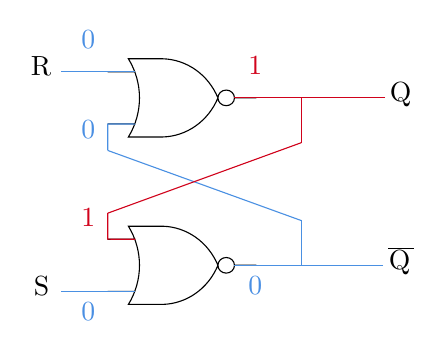
\begin{tikzpicture}[x=0.75pt,y=0.75pt,yscale=-1,xscale=1]
%uncomment if require: \path (0,300); %set diagram left start at 0, and has height of 300

%Shape: Nor Gate [id:dp4086281392337985] 
\draw   (106.27,101.83) -- (122.86,101.83) .. controls (134.43,102.17) and (144.77,109.51) .. (149.4,120.67) .. controls (144.77,131.82) and (134.43,139.16) .. (122.86,139.5) -- (106.27,139.5) .. controls (113.38,127.85) and (113.38,113.49) .. (106.27,101.83) -- cycle (96.31,108.11) -- (109.59,108.11) (96.31,133.22) -- (109.59,133.22) (157.36,120.67) -- (167.98,120.67) (149.4,120.67) .. controls (149.4,118.59) and (151.18,116.9) .. (153.38,116.9) .. controls (155.58,116.9) and (157.36,118.59) .. (157.36,120.67) .. controls (157.36,122.75) and (155.58,124.43) .. (153.38,124.43) .. controls (151.18,124.43) and (149.4,122.75) .. (149.4,120.67) -- cycle ;
%Shape: Nor Gate [id:dp06374716114881951] 
\draw   (106.27,182.5) -- (122.86,182.5) .. controls (134.43,182.84) and (144.77,190.18) .. (149.4,201.33) .. controls (144.77,212.49) and (134.43,219.83) .. (122.86,220.17) -- (106.27,220.17) .. controls (113.38,208.51) and (113.38,194.15) .. (106.27,182.5) -- cycle (96.31,188.78) -- (109.59,188.78) (96.31,213.89) -- (109.59,213.89) (157.36,201.33) -- (167.98,201.33) (149.4,201.33) .. controls (149.4,199.25) and (151.18,197.57) .. (153.38,197.57) .. controls (155.58,197.57) and (157.36,199.25) .. (157.36,201.33) .. controls (157.36,203.41) and (155.58,205.1) .. (153.38,205.1) .. controls (151.18,205.1) and (149.4,203.41) .. (149.4,201.33) -- cycle ;
%Straight Lines [id:da8971344370044351] 
\draw [color={rgb, 255:red, 74; green, 144; blue, 226 }  ,draw opacity=1 ]   (96.31,133.22) -- (96.33,146) ;
%Straight Lines [id:da013829413387980494] 
\draw [color={rgb, 255:red, 208; green, 2; blue, 27 }  ,draw opacity=1 ]   (96.3,176.22) -- (96.31,189) ;
%Straight Lines [id:da2426037289151266] 
\draw [color={rgb, 255:red, 74; green, 144; blue, 226 }  ,draw opacity=1 ]   (109.59,108.11) -- (74,108.11) ;
%Straight Lines [id:da7708764718452497] 
\draw [color={rgb, 255:red, 74; green, 144; blue, 226 }  ,draw opacity=1 ]   (109.59,213.89) -- (74,213.89) ;
%Straight Lines [id:da9929408811615777] 
\draw [color={rgb, 255:red, 208; green, 2; blue, 27 }  ,draw opacity=1 ]   (230,120.67) -- (157.36,120.67) ;
%Straight Lines [id:da9839096117813674] 
\draw [color={rgb, 255:red, 74; green, 144; blue, 226 }  ,draw opacity=1 ]   (229,201.33) -- (157.36,201.33) ;
%Straight Lines [id:da30996716656707235] 
\draw [color={rgb, 255:red, 74; green, 144; blue, 226 }  ,draw opacity=1 ]   (189.5,179.75) -- (96.33,146) ;
%Straight Lines [id:da6058158265884392] 
\draw [color={rgb, 255:red, 74; green, 144; blue, 226 }  ,draw opacity=1 ]   (189.5,179.72) -- (189.5,201.33) ;
%Straight Lines [id:da695661569482763] 
\draw [color={rgb, 255:red, 208; green, 2; blue, 27 }  ,draw opacity=1 ]   (189.5,120.67) -- (189.5,142.28) ;
%Straight Lines [id:da12170141018992597] 
\draw [color={rgb, 255:red, 208; green, 2; blue, 27 }  ,draw opacity=1 ]   (189.5,142.28) -- (96.3,176.22) ;
%Straight Lines [id:da04396196367938876] 
\draw    (231.5,193.33) -- (244,193.33) ;
%Straight Lines [id:da05446462323656964] 
\draw [color={rgb, 255:red, 208; green, 2; blue, 27 }  ,draw opacity=1 ]   (109.59,188.78) -- (96.31,188.75) ;
%Straight Lines [id:da28857795610320724] 
\draw [color={rgb, 255:red, 74; green, 144; blue, 226 }  ,draw opacity=1 ]   (109.59,133.28) -- (96.31,133.25) ;

% Text Node
\draw (231,112.11) node [anchor=north west][inner sep=0.75pt]   [align=left] {Q};
% Text Node
\draw (230.5,192.83) node [anchor=north west][inner sep=0.75pt]   [align=left] {Q};
% Text Node
\draw (58,99.61) node [anchor=north west][inner sep=0.75pt]   [align=left] {R};
% Text Node
\draw (59.5,205.33) node [anchor=north west][inner sep=0.75pt]   [align=left] {S};
% Text Node
\draw (82.31,87.11) node [anchor=north west][inner sep=0.75pt]   [align=left] {\textcolor[rgb]{0.29,0.56,0.89}{0}};
% Text Node
\draw (82.31,217.89) node [anchor=north west][inner sep=0.75pt]   [align=left] {\textcolor[rgb]{0.29,0.56,0.89}{0}};
% Text Node
\draw (162.81,99.67) node [anchor=north west][inner sep=0.75pt]   [align=left] {\textcolor[rgb]{0.82,0.01,0.11}{1}};
% Text Node
\draw (82.31,172.67) node [anchor=north west][inner sep=0.75pt]   [align=left] {\textcolor[rgb]{0.82,0.01,0.11}{1}};
% Text Node
\draw (82.31,130.61) node [anchor=north west][inner sep=0.75pt]   [align=left] {\textcolor[rgb]{0.29,0.56,0.89}{0}};
% Text Node
\draw (162.81,205.39) node [anchor=north west][inner sep=0.75pt]   [align=left] {\textcolor[rgb]{0.29,0.56,0.89}{0}};


\end{tikzpicture}

   			
   			}
   		\end{frame}
   		
   		\begin{frame}
   			\frametitle{NOR SR Latch}
   			\begin{itemize}
   				\item Now, let's see what happens when we feed the latch a positive signal. Specifically, let's give it a value of '1' from the 'R' input.
   				\item We'll see how the resulting value goes from only $Q$ being on to only $\bar{Q}$ being on
   				\item Here's the \textbf{first step}, where we provide R as 1 instead of zero
   			\end{itemize}
   			
   			{
   			\centering
   			

\tikzset{every picture/.style={line width=0.75pt}} %set default line width to 0.75pt        

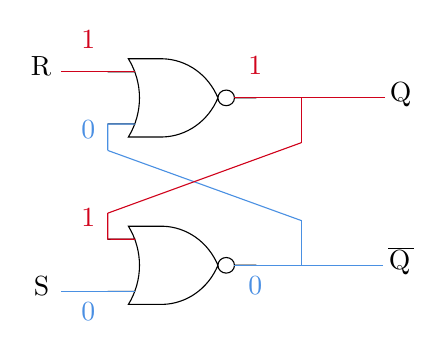
\begin{tikzpicture}[x=0.75pt,y=0.75pt,yscale=-1,xscale=1]
%uncomment if require: \path (0,300); %set diagram left start at 0, and has height of 300

%Shape: Nor Gate [id:dp4086281392337985] 
\draw   (106.27,101.83) -- (122.86,101.83) .. controls (134.43,102.17) and (144.77,109.51) .. (149.4,120.67) .. controls (144.77,131.82) and (134.43,139.16) .. (122.86,139.5) -- (106.27,139.5) .. controls (113.38,127.85) and (113.38,113.49) .. (106.27,101.83) -- cycle (96.31,108.11) -- (109.59,108.11) (96.31,133.22) -- (109.59,133.22) (157.36,120.67) -- (167.98,120.67) (149.4,120.67) .. controls (149.4,118.59) and (151.18,116.9) .. (153.38,116.9) .. controls (155.58,116.9) and (157.36,118.59) .. (157.36,120.67) .. controls (157.36,122.75) and (155.58,124.43) .. (153.38,124.43) .. controls (151.18,124.43) and (149.4,122.75) .. (149.4,120.67) -- cycle ;
%Shape: Nor Gate [id:dp06374716114881951] 
\draw   (106.27,182.5) -- (122.86,182.5) .. controls (134.43,182.84) and (144.77,190.18) .. (149.4,201.33) .. controls (144.77,212.49) and (134.43,219.83) .. (122.86,220.17) -- (106.27,220.17) .. controls (113.38,208.51) and (113.38,194.15) .. (106.27,182.5) -- cycle (96.31,188.78) -- (109.59,188.78) (96.31,213.89) -- (109.59,213.89) (157.36,201.33) -- (167.98,201.33) (149.4,201.33) .. controls (149.4,199.25) and (151.18,197.57) .. (153.38,197.57) .. controls (155.58,197.57) and (157.36,199.25) .. (157.36,201.33) .. controls (157.36,203.41) and (155.58,205.1) .. (153.38,205.1) .. controls (151.18,205.1) and (149.4,203.41) .. (149.4,201.33) -- cycle ;
%Straight Lines [id:da8971344370044351] 
\draw [color={rgb, 255:red, 74; green, 144; blue, 226 }  ,draw opacity=1 ]   (96.31,133.22) -- (96.33,146) ;
%Straight Lines [id:da013829413387980494] 
\draw [color={rgb, 255:red, 208; green, 2; blue, 27 }  ,draw opacity=1 ]   (96.3,176.22) -- (96.31,189) ;
%Straight Lines [id:da2426037289151266] 
\draw [color={rgb, 255:red, 208; green, 2; blue, 27 }  ,draw opacity=1 ]   (109.59,108.11) -- (74,108.11) ;
%Straight Lines [id:da7708764718452497] 
\draw [color={rgb, 255:red, 74; green, 144; blue, 226 }  ,draw opacity=1 ]   (109.59,213.89) -- (74,213.89) ;
%Straight Lines [id:da9929408811615777] 
\draw [color={rgb, 255:red, 208; green, 2; blue, 27 }  ,draw opacity=1 ]   (230,120.67) -- (157.36,120.67) ;
%Straight Lines [id:da9839096117813674] 
\draw [color={rgb, 255:red, 74; green, 144; blue, 226 }  ,draw opacity=1 ]   (229,201.33) -- (157.36,201.33) ;
%Straight Lines [id:da30996716656707235] 
\draw [color={rgb, 255:red, 74; green, 144; blue, 226 }  ,draw opacity=1 ]   (189.5,179.75) -- (96.33,146) ;
%Straight Lines [id:da6058158265884392] 
\draw [color={rgb, 255:red, 74; green, 144; blue, 226 }  ,draw opacity=1 ]   (189.5,179.72) -- (189.5,201.33) ;
%Straight Lines [id:da695661569482763] 
\draw [color={rgb, 255:red, 208; green, 2; blue, 27 }  ,draw opacity=1 ]   (189.5,120.67) -- (189.5,142.28) ;
%Straight Lines [id:da12170141018992597] 
\draw [color={rgb, 255:red, 208; green, 2; blue, 27 }  ,draw opacity=1 ]   (189.5,142.28) -- (96.3,176.22) ;
%Straight Lines [id:da04396196367938876] 
\draw    (231.5,193.33) -- (244,193.33) ;
%Straight Lines [id:da05446462323656964] 
\draw [color={rgb, 255:red, 208; green, 2; blue, 27 }  ,draw opacity=1 ]   (109.59,188.78) -- (96.31,188.75) ;
%Straight Lines [id:da28857795610320724] 
\draw [color={rgb, 255:red, 74; green, 144; blue, 226 }  ,draw opacity=1 ]   (109.59,133.28) -- (96.31,133.25) ;

% Text Node
\draw (231,112.11) node [anchor=north west][inner sep=0.75pt]   [align=left] {Q};
% Text Node
\draw (230.5,192.83) node [anchor=north west][inner sep=0.75pt]   [align=left] {Q};
% Text Node
\draw (58,99.61) node [anchor=north west][inner sep=0.75pt]   [align=left] {R};
% Text Node
\draw (59.5,205.33) node [anchor=north west][inner sep=0.75pt]   [align=left] {S};
% Text Node
\draw (82.31,87.11) node [anchor=north west][inner sep=0.75pt]   [align=left] {\textcolor[rgb]{0.82,0.01,0.11}{1}};
% Text Node
\draw (82.31,217.89) node [anchor=north west][inner sep=0.75pt]   [align=left] {\textcolor[rgb]{0.29,0.56,0.89}{0}};
% Text Node
\draw (162.81,99.67) node [anchor=north west][inner sep=0.75pt]   [align=left] {\textcolor[rgb]{0.82,0.01,0.11}{1}};
% Text Node
\draw (82.31,172.67) node [anchor=north west][inner sep=0.75pt]   [align=left] {\textcolor[rgb]{0.82,0.01,0.11}{1}};
% Text Node
\draw (82.31,130.61) node [anchor=north west][inner sep=0.75pt]   [align=left] {\textcolor[rgb]{0.29,0.56,0.89}{0}};
% Text Node
\draw (162.81,205.39) node [anchor=north west][inner sep=0.75pt]   [align=left] {\textcolor[rgb]{0.29,0.56,0.89}{0}};


\end{tikzpicture}

   			}
   			
   			
   		\end{frame}
   		
   		\begin{frame}
   			\frametitle{NOR SR Latch}
   			\begin{itemize}
   				\item Here's the \textbf{second step}, where the result of the \texttt{NOR} gate up top propagates down to the other \texttt{NOR} gate.
   			\end{itemize}
   			
   			{
   			\centering
   			

\tikzset{every picture/.style={line width=0.75pt}} %set default line width to 0.75pt        

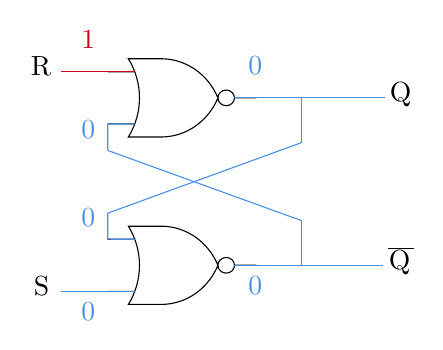
\begin{tikzpicture}[x=0.75pt,y=0.75pt,yscale=-1,xscale=1]
%uncomment if require: \path (0,300); %set diagram left start at 0, and has height of 300

%Shape: Nor Gate [id:dp4086281392337985] 
\draw   (106.27,101.83) -- (122.86,101.83) .. controls (134.43,102.17) and (144.77,109.51) .. (149.4,120.67) .. controls (144.77,131.82) and (134.43,139.16) .. (122.86,139.5) -- (106.27,139.5) .. controls (113.38,127.85) and (113.38,113.49) .. (106.27,101.83) -- cycle (96.31,108.11) -- (109.59,108.11) (96.31,133.22) -- (109.59,133.22) (157.36,120.67) -- (167.98,120.67) (149.4,120.67) .. controls (149.4,118.59) and (151.18,116.9) .. (153.38,116.9) .. controls (155.58,116.9) and (157.36,118.59) .. (157.36,120.67) .. controls (157.36,122.75) and (155.58,124.43) .. (153.38,124.43) .. controls (151.18,124.43) and (149.4,122.75) .. (149.4,120.67) -- cycle ;
%Shape: Nor Gate [id:dp06374716114881951] 
\draw   (106.27,182.5) -- (122.86,182.5) .. controls (134.43,182.84) and (144.77,190.18) .. (149.4,201.33) .. controls (144.77,212.49) and (134.43,219.83) .. (122.86,220.17) -- (106.27,220.17) .. controls (113.38,208.51) and (113.38,194.15) .. (106.27,182.5) -- cycle (96.31,188.78) -- (109.59,188.78) (96.31,213.89) -- (109.59,213.89) (157.36,201.33) -- (167.98,201.33) (149.4,201.33) .. controls (149.4,199.25) and (151.18,197.57) .. (153.38,197.57) .. controls (155.58,197.57) and (157.36,199.25) .. (157.36,201.33) .. controls (157.36,203.41) and (155.58,205.1) .. (153.38,205.1) .. controls (151.18,205.1) and (149.4,203.41) .. (149.4,201.33) -- cycle ;
%Straight Lines [id:da8971344370044351] 
\draw [color={rgb, 255:red, 74; green, 144; blue, 226 }  ,draw opacity=1 ]   (96.31,133.22) -- (96.33,146) ;
%Straight Lines [id:da013829413387980494] 
\draw [color={rgb, 255:red, 74; green, 144; blue, 226 }  ,draw opacity=1 ]   (96.3,176.22) -- (96.31,189) ;
%Straight Lines [id:da2426037289151266] 
\draw [color={rgb, 255:red, 208; green, 2; blue, 27 }  ,draw opacity=1 ]   (109.59,108.11) -- (74,108.11) ;
%Straight Lines [id:da7708764718452497] 
\draw [color={rgb, 255:red, 74; green, 144; blue, 226 }  ,draw opacity=1 ]   (109.59,213.89) -- (74,213.89) ;
%Straight Lines [id:da9929408811615777] 
\draw [color={rgb, 255:red, 74; green, 144; blue, 226 }  ,draw opacity=1 ]   (230,120.67) -- (157.36,120.67) ;
%Straight Lines [id:da9839096117813674] 
\draw [color={rgb, 255:red, 74; green, 144; blue, 226 }  ,draw opacity=1 ]   (229,201.33) -- (157.36,201.33) ;
%Straight Lines [id:da30996716656707235] 
\draw [color={rgb, 255:red, 74; green, 144; blue, 226 }  ,draw opacity=1 ]   (189.5,179.75) -- (96.33,146) ;
%Straight Lines [id:da6058158265884392] 
\draw [color={rgb, 255:red, 74; green, 144; blue, 226 }  ,draw opacity=1 ]   (189.5,179.72) -- (189.5,201.33) ;
%Straight Lines [id:da695661569482763] 
\draw [color={rgb, 255:red, 74; green, 144; blue, 226 }  ,draw opacity=1 ]   (189.5,120.67) -- (189.5,142.28) ;
%Straight Lines [id:da12170141018992597] 
\draw [color={rgb, 255:red, 74; green, 144; blue, 226 }  ,draw opacity=1 ]   (189.5,142.28) -- (96.3,176.22) ;
%Straight Lines [id:da04396196367938876] 
\draw    (231.5,193.33) -- (244,193.33) ;
%Straight Lines [id:da05446462323656964] 
\draw [color={rgb, 255:red, 74; green, 144; blue, 226 }  ,draw opacity=1 ]   (109.59,188.78) -- (96.31,188.75) ;
%Straight Lines [id:da28857795610320724] 
\draw [color={rgb, 255:red, 74; green, 144; blue, 226 }  ,draw opacity=1 ]   (109.59,133.28) -- (96.31,133.25) ;

% Text Node
\draw (231,112.11) node [anchor=north west][inner sep=0.75pt]   [align=left] {Q};
% Text Node
\draw (230.5,192.83) node [anchor=north west][inner sep=0.75pt]   [align=left] {Q};
% Text Node
\draw (58,99.61) node [anchor=north west][inner sep=0.75pt]   [align=left] {R};
% Text Node
\draw (59.5,205.33) node [anchor=north west][inner sep=0.75pt]   [align=left] {S};
% Text Node
\draw (82.31,87.11) node [anchor=north west][inner sep=0.75pt]   [align=left] {\textcolor[rgb]{0.82,0.01,0.11}{1}};
% Text Node
\draw (82.31,217.89) node [anchor=north west][inner sep=0.75pt]   [align=left] {\textcolor[rgb]{0.29,0.56,0.89}{0}};
% Text Node
\draw (162.81,99.67) node [anchor=north west][inner sep=0.75pt]   [align=left] {\textcolor[rgb]{0.29,0.56,0.89}{0}};
% Text Node
\draw (82.31,172.67) node [anchor=north west][inner sep=0.75pt]   [align=left] {\textcolor[rgb]{0.29,0.56,0.89}{0}};
% Text Node
\draw (82.31,130.61) node [anchor=north west][inner sep=0.75pt]   [align=left] {\textcolor[rgb]{0.29,0.56,0.89}{0}};
% Text Node
\draw (162.81,205.39) node [anchor=north west][inner sep=0.75pt]   [align=left] {\textcolor[rgb]{0.29,0.56,0.89}{0}};


\end{tikzpicture}

   			
   			}
   		\end{frame}
   		
   		\begin{frame}
   			\frametitle{NOR SR Latch}
   			\begin{itemize}
   				\item Here's the third and \textbf{final step}. Finally, the result coming out of the bottom \texttt{NOR} gate alters the output coming and pointing to $\bar{Q}$
   			\end{itemize}
   			
   			{
   			\centering
   			

\tikzset{every picture/.style={line width=0.75pt}} %set default line width to 0.75pt        

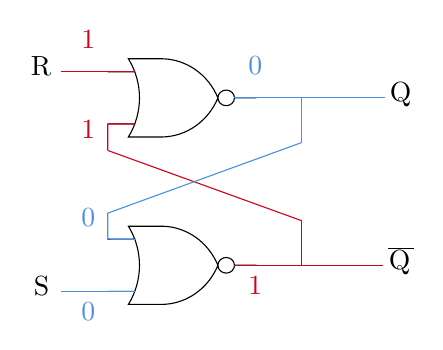
\begin{tikzpicture}[x=0.75pt,y=0.75pt,yscale=-1,xscale=1]
%uncomment if require: \path (0,300); %set diagram left start at 0, and has height of 300

%Shape: Nor Gate [id:dp4086281392337985] 
\draw   (106.27,101.83) -- (122.86,101.83) .. controls (134.43,102.17) and (144.77,109.51) .. (149.4,120.67) .. controls (144.77,131.82) and (134.43,139.16) .. (122.86,139.5) -- (106.27,139.5) .. controls (113.38,127.85) and (113.38,113.49) .. (106.27,101.83) -- cycle (96.31,108.11) -- (109.59,108.11) (96.31,133.22) -- (109.59,133.22) (157.36,120.67) -- (167.98,120.67) (149.4,120.67) .. controls (149.4,118.59) and (151.18,116.9) .. (153.38,116.9) .. controls (155.58,116.9) and (157.36,118.59) .. (157.36,120.67) .. controls (157.36,122.75) and (155.58,124.43) .. (153.38,124.43) .. controls (151.18,124.43) and (149.4,122.75) .. (149.4,120.67) -- cycle ;
%Shape: Nor Gate [id:dp06374716114881951] 
\draw   (106.27,182.5) -- (122.86,182.5) .. controls (134.43,182.84) and (144.77,190.18) .. (149.4,201.33) .. controls (144.77,212.49) and (134.43,219.83) .. (122.86,220.17) -- (106.27,220.17) .. controls (113.38,208.51) and (113.38,194.15) .. (106.27,182.5) -- cycle (96.31,188.78) -- (109.59,188.78) (96.31,213.89) -- (109.59,213.89) (157.36,201.33) -- (167.98,201.33) (149.4,201.33) .. controls (149.4,199.25) and (151.18,197.57) .. (153.38,197.57) .. controls (155.58,197.57) and (157.36,199.25) .. (157.36,201.33) .. controls (157.36,203.41) and (155.58,205.1) .. (153.38,205.1) .. controls (151.18,205.1) and (149.4,203.41) .. (149.4,201.33) -- cycle ;
%Straight Lines [id:da8971344370044351] 
\draw [color={rgb, 255:red, 208; green, 2; blue, 27 }  ,draw opacity=1 ]   (96.31,133.22) -- (96.33,146) ;
%Straight Lines [id:da013829413387980494] 
\draw [color={rgb, 255:red, 74; green, 144; blue, 226 }  ,draw opacity=1 ]   (96.3,176.22) -- (96.31,189) ;
%Straight Lines [id:da2426037289151266] 
\draw [color={rgb, 255:red, 208; green, 2; blue, 27 }  ,draw opacity=1 ]   (109.59,108.11) -- (74,108.11) ;
%Straight Lines [id:da7708764718452497] 
\draw [color={rgb, 255:red, 74; green, 144; blue, 226 }  ,draw opacity=1 ]   (109.59,213.89) -- (74,213.89) ;
%Straight Lines [id:da9929408811615777] 
\draw [color={rgb, 255:red, 74; green, 144; blue, 226 }  ,draw opacity=1 ]   (230,120.67) -- (157.36,120.67) ;
%Straight Lines [id:da9839096117813674] 
\draw [color={rgb, 255:red, 208; green, 2; blue, 27 }  ,draw opacity=1 ]   (229,201.33) -- (157.36,201.33) ;
%Straight Lines [id:da30996716656707235] 
\draw [color={rgb, 255:red, 208; green, 2; blue, 27 }  ,draw opacity=1 ]   (189.5,179.75) -- (96.33,146) ;
%Straight Lines [id:da6058158265884392] 
\draw [color={rgb, 255:red, 208; green, 2; blue, 27 }  ,draw opacity=1 ]   (189.5,179.72) -- (189.5,201.33) ;
%Straight Lines [id:da695661569482763] 
\draw [color={rgb, 255:red, 74; green, 144; blue, 226 }  ,draw opacity=1 ]   (189.5,120.67) -- (189.5,142.28) ;
%Straight Lines [id:da12170141018992597] 
\draw [color={rgb, 255:red, 74; green, 144; blue, 226 }  ,draw opacity=1 ]   (189.5,142.28) -- (96.3,176.22) ;
%Straight Lines [id:da04396196367938876] 
\draw    (231.5,193.33) -- (244,193.33) ;
%Straight Lines [id:da05446462323656964] 
\draw [color={rgb, 255:red, 74; green, 144; blue, 226 }  ,draw opacity=1 ]   (109.59,188.78) -- (96.31,188.75) ;
%Straight Lines [id:da28857795610320724] 
\draw [color={rgb, 255:red, 208; green, 2; blue, 27 }  ,draw opacity=1 ]   (109.59,133.28) -- (96.31,133.25) ;

% Text Node
\draw (231,112.11) node [anchor=north west][inner sep=0.75pt]   [align=left] {Q};
% Text Node
\draw (230.5,192.83) node [anchor=north west][inner sep=0.75pt]   [align=left] {Q};
% Text Node
\draw (58,99.61) node [anchor=north west][inner sep=0.75pt]   [align=left] {R};
% Text Node
\draw (59.5,205.33) node [anchor=north west][inner sep=0.75pt]   [align=left] {S};
% Text Node
\draw (82.31,87.11) node [anchor=north west][inner sep=0.75pt]   [align=left] {\textcolor[rgb]{0.82,0.01,0.11}{1}};
% Text Node
\draw (82.31,217.89) node [anchor=north west][inner sep=0.75pt]   [align=left] {\textcolor[rgb]{0.29,0.56,0.89}{0}};
% Text Node
\draw (162.81,99.67) node [anchor=north west][inner sep=0.75pt]   [align=left] {\textcolor[rgb]{0.29,0.56,0.89}{0}};
% Text Node
\draw (82.31,172.67) node [anchor=north west][inner sep=0.75pt]   [align=left] {\textcolor[rgb]{0.29,0.56,0.89}{0}};
% Text Node
\draw (82.31,130.61) node [anchor=north west][inner sep=0.75pt]   [align=left] {\textcolor[rgb]{0.82,0.01,0.11}{1}};
% Text Node
\draw (162.81,205.39) node [anchor=north west][inner sep=0.75pt]   [align=left] {\textcolor[rgb]{0.82,0.01,0.11}{1}};


\end{tikzpicture}

   			}
   			
   		\end{frame}
   		
   		\begin{frame}
   			\frametitle{NOR SR Latch}
   			\begin{itemize}
   				\item Note that if we remove the 1 coming in from R at this point, the output states will stay the exact same.
   			\end{itemize}
   			
   			{
   			\centering
   				

\tikzset{every picture/.style={line width=0.75pt}} %set default line width to 0.75pt        

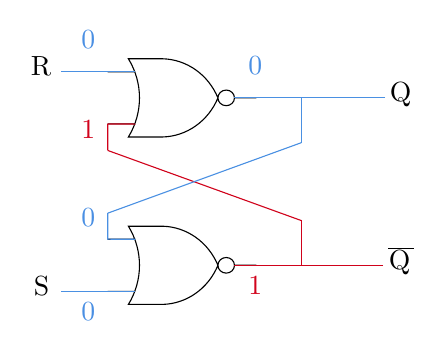
\begin{tikzpicture}[x=0.75pt,y=0.75pt,yscale=-1,xscale=1]
%uncomment if require: \path (0,300); %set diagram left start at 0, and has height of 300

%Shape: Nor Gate [id:dp4086281392337985] 
\draw   (106.27,101.83) -- (122.86,101.83) .. controls (134.43,102.17) and (144.77,109.51) .. (149.4,120.67) .. controls (144.77,131.82) and (134.43,139.16) .. (122.86,139.5) -- (106.27,139.5) .. controls (113.38,127.85) and (113.38,113.49) .. (106.27,101.83) -- cycle (96.31,108.11) -- (109.59,108.11) (96.31,133.22) -- (109.59,133.22) (157.36,120.67) -- (167.98,120.67) (149.4,120.67) .. controls (149.4,118.59) and (151.18,116.9) .. (153.38,116.9) .. controls (155.58,116.9) and (157.36,118.59) .. (157.36,120.67) .. controls (157.36,122.75) and (155.58,124.43) .. (153.38,124.43) .. controls (151.18,124.43) and (149.4,122.75) .. (149.4,120.67) -- cycle ;
%Shape: Nor Gate [id:dp06374716114881951] 
\draw   (106.27,182.5) -- (122.86,182.5) .. controls (134.43,182.84) and (144.77,190.18) .. (149.4,201.33) .. controls (144.77,212.49) and (134.43,219.83) .. (122.86,220.17) -- (106.27,220.17) .. controls (113.38,208.51) and (113.38,194.15) .. (106.27,182.5) -- cycle (96.31,188.78) -- (109.59,188.78) (96.31,213.89) -- (109.59,213.89) (157.36,201.33) -- (167.98,201.33) (149.4,201.33) .. controls (149.4,199.25) and (151.18,197.57) .. (153.38,197.57) .. controls (155.58,197.57) and (157.36,199.25) .. (157.36,201.33) .. controls (157.36,203.41) and (155.58,205.1) .. (153.38,205.1) .. controls (151.18,205.1) and (149.4,203.41) .. (149.4,201.33) -- cycle ;
%Straight Lines [id:da8971344370044351] 
\draw [color={rgb, 255:red, 208; green, 2; blue, 27 }  ,draw opacity=1 ]   (96.31,133.22) -- (96.33,146) ;
%Straight Lines [id:da013829413387980494] 
\draw [color={rgb, 255:red, 74; green, 144; blue, 226 }  ,draw opacity=1 ]   (96.3,176.22) -- (96.31,189) ;
%Straight Lines [id:da2426037289151266] 
\draw [color={rgb, 255:red, 74; green, 144; blue, 226 }  ,draw opacity=1 ]   (109.59,108.11) -- (74,108.11) ;
%Straight Lines [id:da7708764718452497] 
\draw [color={rgb, 255:red, 74; green, 144; blue, 226 }  ,draw opacity=1 ]   (109.59,213.89) -- (74,213.89) ;
%Straight Lines [id:da9929408811615777] 
\draw [color={rgb, 255:red, 74; green, 144; blue, 226 }  ,draw opacity=1 ]   (230,120.67) -- (157.36,120.67) ;
%Straight Lines [id:da9839096117813674] 
\draw [color={rgb, 255:red, 208; green, 2; blue, 27 }  ,draw opacity=1 ]   (229,201.33) -- (157.36,201.33) ;
%Straight Lines [id:da30996716656707235] 
\draw [color={rgb, 255:red, 208; green, 2; blue, 27 }  ,draw opacity=1 ]   (189.5,179.75) -- (96.33,146) ;
%Straight Lines [id:da6058158265884392] 
\draw [color={rgb, 255:red, 208; green, 2; blue, 27 }  ,draw opacity=1 ]   (189.5,179.72) -- (189.5,201.33) ;
%Straight Lines [id:da695661569482763] 
\draw [color={rgb, 255:red, 74; green, 144; blue, 226 }  ,draw opacity=1 ]   (189.5,120.67) -- (189.5,142.28) ;
%Straight Lines [id:da12170141018992597] 
\draw [color={rgb, 255:red, 74; green, 144; blue, 226 }  ,draw opacity=1 ]   (189.5,142.28) -- (96.3,176.22) ;
%Straight Lines [id:da04396196367938876] 
\draw    (231.5,193.33) -- (244,193.33) ;
%Straight Lines [id:da05446462323656964] 
\draw [color={rgb, 255:red, 74; green, 144; blue, 226 }  ,draw opacity=1 ]   (109.59,188.78) -- (96.31,188.75) ;
%Straight Lines [id:da28857795610320724] 
\draw [color={rgb, 255:red, 208; green, 2; blue, 27 }  ,draw opacity=1 ]   (109.59,133.28) -- (96.31,133.25) ;

% Text Node
\draw (231,112.11) node [anchor=north west][inner sep=0.75pt]   [align=left] {Q};
% Text Node
\draw (230.5,192.83) node [anchor=north west][inner sep=0.75pt]   [align=left] {Q};
% Text Node
\draw (58,99.61) node [anchor=north west][inner sep=0.75pt]   [align=left] {R};
% Text Node
\draw (59.5,205.33) node [anchor=north west][inner sep=0.75pt]   [align=left] {S};
% Text Node
\draw (82.31,87.11) node [anchor=north west][inner sep=0.75pt]   [align=left] {\textcolor[rgb]{0.29,0.56,0.89}{0}};
% Text Node
\draw (82.31,217.89) node [anchor=north west][inner sep=0.75pt]   [align=left] {\textcolor[rgb]{0.29,0.56,0.89}{0}};
% Text Node
\draw (162.81,99.67) node [anchor=north west][inner sep=0.75pt]   [align=left] {\textcolor[rgb]{0.29,0.56,0.89}{0}};
% Text Node
\draw (82.31,172.67) node [anchor=north west][inner sep=0.75pt]   [align=left] {\textcolor[rgb]{0.29,0.56,0.89}{0}};
% Text Node
\draw (82.31,130.61) node [anchor=north west][inner sep=0.75pt]   [align=left] {\textcolor[rgb]{0.82,0.01,0.11}{1}};
% Text Node
\draw (162.81,205.39) node [anchor=north west][inner sep=0.75pt]   [align=left] {\textcolor[rgb]{0.82,0.01,0.11}{1}};


\end{tikzpicture}

   			}
   			
   			\begin{itemize}
   				\item This is the beauty of latches- they can keep a state for us without us having to keep a signal coming in consistently.
   				\item Circuits like this are the basis for sequential logic.
   			\end{itemize}
   			
   			
   		\end{frame}
   		
   		\begin{frame}
   			\frametitle{Other Types of Latches}
   			\begin{itemize}
   				\item First of all, you can make an equivalent latch to the NOR SR Latch by using \texttt{NAND} gates. It's basically functionally the same as the NOR SR Latch.
   				\item Additionally, there are other types of Latches. Again, since this is a 1-credit class, this is the one type of latch that we'll be going over in-depth.
   				\item If you want to learn more about latches, we'll be posting some stuff on the course website for you to check out.
   			\end{itemize}
   		\end{frame}
   		
   	\section{Flip Flops}
   	
   	\begin{frame}
                \vfill
                \centering
                \begin{beamercolorbox}[sep=8pt,center,shadow=true,rounded=true]{title}
                    \usebeamerfont{title}Flip Flops and Clocks\par%
                \end{beamercolorbox}
                \vfill
             \end{frame}
   	
   		\begin{frame}
   			\frametitle{What's a Flip Flop?}
   			\begin{itemize}
   				\item Certainly not a type of shoe you'd wear to the beach.
   				\item In a sentence, Flip Flops are basically just latches which are only usable when you give a 'control' input is on.
   				\item That may sound silly, but it helps when we want to update memory at certain times
   			\end{itemize}
   		\end{frame}
   		
   		\begin{frame}
   			\frametitle{What's a Flip Flop?}
   			\begin{itemize}
   				\item Let's say you wanted your latch(es) to update, but only when you were certain that the inputs for your latch(es) were for sure decided?
   				\item Using a flip flop instead of your latches will only allow the latches to change when that 'control' input switches to on, letting it know that it's okay to update
   				\item If you're having trouble imagining this, think of why we set our test delays to 2+ seconds instead of having them run with no delay
   			\end{itemize}
   		\end{frame}
   		
   		\subsection{Flip Flops vs. Latches}
   		
   		\begin{frame}
   			\frametitle{How does that end up looking?}
   			\begin{itemize}
   				\item Let's look at a Flip Flop and a Latch, side by side.
   				\item First, here's a plain old latch.
   			\end{itemize}
   			
   			{
   			\centering
				\tikzset{every picture/.style={line width=0.75pt}} %set default line width to 0.75pt        

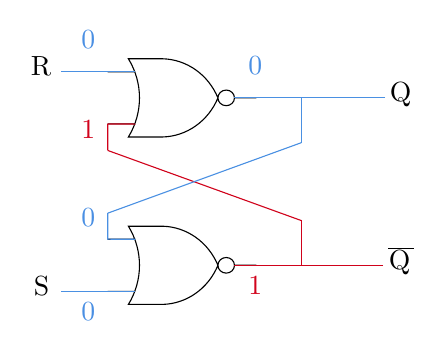
\begin{tikzpicture}[x=0.75pt,y=0.75pt,yscale=-1,xscale=1]
%uncomment if require: \path (0,300); %set diagram left start at 0, and has height of 300

%Shape: Nor Gate [id:dp4086281392337985] 
\draw   (106.27,101.83) -- (122.86,101.83) .. controls (134.43,102.17) and (144.77,109.51) .. (149.4,120.67) .. controls (144.77,131.82) and (134.43,139.16) .. (122.86,139.5) -- (106.27,139.5) .. controls (113.38,127.85) and (113.38,113.49) .. (106.27,101.83) -- cycle (96.31,108.11) -- (109.59,108.11) (96.31,133.22) -- (109.59,133.22) (157.36,120.67) -- (167.98,120.67) (149.4,120.67) .. controls (149.4,118.59) and (151.18,116.9) .. (153.38,116.9) .. controls (155.58,116.9) and (157.36,118.59) .. (157.36,120.67) .. controls (157.36,122.75) and (155.58,124.43) .. (153.38,124.43) .. controls (151.18,124.43) and (149.4,122.75) .. (149.4,120.67) -- cycle ;
%Shape: Nor Gate [id:dp06374716114881951] 
\draw   (106.27,182.5) -- (122.86,182.5) .. controls (134.43,182.84) and (144.77,190.18) .. (149.4,201.33) .. controls (144.77,212.49) and (134.43,219.83) .. (122.86,220.17) -- (106.27,220.17) .. controls (113.38,208.51) and (113.38,194.15) .. (106.27,182.5) -- cycle (96.31,188.78) -- (109.59,188.78) (96.31,213.89) -- (109.59,213.89) (157.36,201.33) -- (167.98,201.33) (149.4,201.33) .. controls (149.4,199.25) and (151.18,197.57) .. (153.38,197.57) .. controls (155.58,197.57) and (157.36,199.25) .. (157.36,201.33) .. controls (157.36,203.41) and (155.58,205.1) .. (153.38,205.1) .. controls (151.18,205.1) and (149.4,203.41) .. (149.4,201.33) -- cycle ;
%Straight Lines [id:da8971344370044351] 
\draw [color={rgb, 255:red, 208; green, 2; blue, 27 }  ,draw opacity=1 ]   (96.31,133.22) -- (96.33,146) ;
%Straight Lines [id:da013829413387980494] 
\draw [color={rgb, 255:red, 74; green, 144; blue, 226 }  ,draw opacity=1 ]   (96.3,176.22) -- (96.31,189) ;
%Straight Lines [id:da2426037289151266] 
\draw [color={rgb, 255:red, 74; green, 144; blue, 226 }  ,draw opacity=1 ]   (109.59,108.11) -- (74,108.11) ;
%Straight Lines [id:da7708764718452497] 
\draw [color={rgb, 255:red, 74; green, 144; blue, 226 }  ,draw opacity=1 ]   (109.59,213.89) -- (74,213.89) ;
%Straight Lines [id:da9929408811615777] 
\draw [color={rgb, 255:red, 74; green, 144; blue, 226 }  ,draw opacity=1 ]   (230,120.67) -- (157.36,120.67) ;
%Straight Lines [id:da9839096117813674] 
\draw [color={rgb, 255:red, 208; green, 2; blue, 27 }  ,draw opacity=1 ]   (229,201.33) -- (157.36,201.33) ;
%Straight Lines [id:da30996716656707235] 
\draw [color={rgb, 255:red, 208; green, 2; blue, 27 }  ,draw opacity=1 ]   (189.5,179.75) -- (96.33,146) ;
%Straight Lines [id:da6058158265884392] 
\draw [color={rgb, 255:red, 208; green, 2; blue, 27 }  ,draw opacity=1 ]   (189.5,179.72) -- (189.5,201.33) ;
%Straight Lines [id:da695661569482763] 
\draw [color={rgb, 255:red, 74; green, 144; blue, 226 }  ,draw opacity=1 ]   (189.5,120.67) -- (189.5,142.28) ;
%Straight Lines [id:da12170141018992597] 
\draw [color={rgb, 255:red, 74; green, 144; blue, 226 }  ,draw opacity=1 ]   (189.5,142.28) -- (96.3,176.22) ;
%Straight Lines [id:da04396196367938876] 
\draw    (231.5,193.33) -- (244,193.33) ;
%Straight Lines [id:da05446462323656964] 
\draw [color={rgb, 255:red, 74; green, 144; blue, 226 }  ,draw opacity=1 ]   (109.59,188.78) -- (96.31,188.75) ;
%Straight Lines [id:da28857795610320724] 
\draw [color={rgb, 255:red, 208; green, 2; blue, 27 }  ,draw opacity=1 ]   (109.59,133.28) -- (96.31,133.25) ;

% Text Node
\draw (231,112.11) node [anchor=north west][inner sep=0.75pt]   [align=left] {Q};
% Text Node
\draw (230.5,192.83) node [anchor=north west][inner sep=0.75pt]   [align=left] {Q};
% Text Node
\draw (58,99.61) node [anchor=north west][inner sep=0.75pt]   [align=left] {R};
% Text Node
\draw (59.5,205.33) node [anchor=north west][inner sep=0.75pt]   [align=left] {S};
% Text Node
\draw (82.31,87.11) node [anchor=north west][inner sep=0.75pt]   [align=left] {\textcolor[rgb]{0.29,0.56,0.89}{0}};
% Text Node
\draw (82.31,217.89) node [anchor=north west][inner sep=0.75pt]   [align=left] {\textcolor[rgb]{0.29,0.56,0.89}{0}};
% Text Node
\draw (162.81,99.67) node [anchor=north west][inner sep=0.75pt]   [align=left] {\textcolor[rgb]{0.29,0.56,0.89}{0}};
% Text Node
\draw (82.31,172.67) node [anchor=north west][inner sep=0.75pt]   [align=left] {\textcolor[rgb]{0.29,0.56,0.89}{0}};
% Text Node
\draw (82.31,130.61) node [anchor=north west][inner sep=0.75pt]   [align=left] {\textcolor[rgb]{0.82,0.01,0.11}{1}};
% Text Node
\draw (162.81,205.39) node [anchor=north west][inner sep=0.75pt]   [align=left] {\textcolor[rgb]{0.82,0.01,0.11}{1}};


\end{tikzpicture}   			
   			
   			}
   		\end{frame}
   		
   		\begin{frame}
   			\frametitle{How does that end up looking?}
   			\begin{itemize}
   				\item And here's the flip flop version.
   			\end{itemize}
   			
   			{
   			\centering
   			

\tikzset{every picture/.style={line width=0.75pt}} %set default line width to 0.75pt        

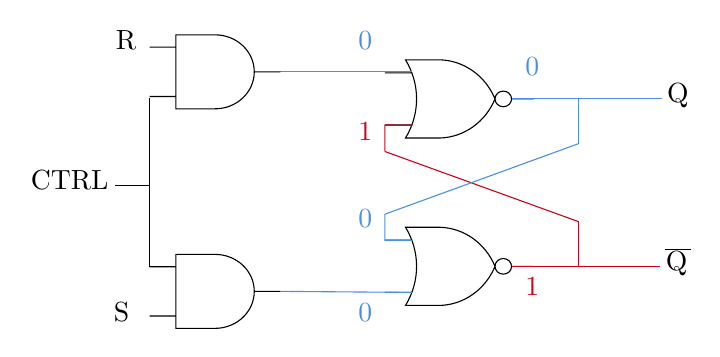
\begin{tikzpicture}[x=0.75pt,y=0.75pt,yscale=-1,xscale=1]
%uncomment if require: \path (0,300); %set diagram left start at 0, and has height of 300

%Shape: Nor Gate [id:dp20115173758169524] 
\draw   (348.77,100.33) -- (365.36,100.33) .. controls (376.93,100.67) and (387.27,108.01) .. (391.9,119.17) .. controls (387.27,130.32) and (376.93,137.66) .. (365.36,138) -- (348.77,138) .. controls (355.88,126.35) and (355.88,111.99) .. (348.77,100.33) -- cycle (338.81,106.61) -- (352.09,106.61) (338.81,131.72) -- (352.09,131.72) (399.86,119.17) -- (410.48,119.17) (391.9,119.17) .. controls (391.9,117.09) and (393.68,115.4) .. (395.88,115.4) .. controls (398.08,115.4) and (399.86,117.09) .. (399.86,119.17) .. controls (399.86,121.25) and (398.08,122.93) .. (395.88,122.93) .. controls (393.68,122.93) and (391.9,121.25) .. (391.9,119.17) -- cycle ;
%Shape: Nor Gate [id:dp3323560999277514] 
\draw   (348.77,181) -- (365.36,181) .. controls (376.93,181.34) and (387.27,188.68) .. (391.9,199.83) .. controls (387.27,210.99) and (376.93,218.33) .. (365.36,218.67) -- (348.77,218.67) .. controls (355.88,207.01) and (355.88,192.65) .. (348.77,181) -- cycle (338.81,187.28) -- (352.09,187.28) (338.81,212.39) -- (352.09,212.39) (399.86,199.83) -- (410.48,199.83) (391.9,199.83) .. controls (391.9,197.75) and (393.68,196.07) .. (395.88,196.07) .. controls (398.08,196.07) and (399.86,197.75) .. (399.86,199.83) .. controls (399.86,201.91) and (398.08,203.6) .. (395.88,203.6) .. controls (393.68,203.6) and (391.9,201.91) .. (391.9,199.83) -- cycle ;
%Straight Lines [id:da20536033587018832] 
\draw [color={rgb, 255:red, 208; green, 2; blue, 27 }  ,draw opacity=1 ]   (338.81,131.72) -- (338.83,144.5) ;
%Straight Lines [id:da7971122968837543] 
\draw [color={rgb, 255:red, 74; green, 144; blue, 226 }  ,draw opacity=1 ]   (338.8,174.72) -- (338.81,187.5) ;
%Straight Lines [id:da4518253411889239] 
\draw [color={rgb, 255:red, 74; green, 144; blue, 226 }  ,draw opacity=1 ]   (352.09,106.11) -- (288.5,106.11) ;
%Straight Lines [id:da9993575054775435] 
\draw [color={rgb, 255:red, 74; green, 144; blue, 226 }  ,draw opacity=1 ]   (352.09,212.39) -- (288.5,211.89) ;
%Straight Lines [id:da8660645046667792] 
\draw [color={rgb, 255:red, 74; green, 144; blue, 226 }  ,draw opacity=1 ]   (472.5,119.17) -- (399.86,119.17) ;
%Straight Lines [id:da7554560655091269] 
\draw [color={rgb, 255:red, 208; green, 2; blue, 27 }  ,draw opacity=1 ]   (471.5,199.83) -- (399.86,199.83) ;
%Straight Lines [id:da261243510360913] 
\draw [color={rgb, 255:red, 208; green, 2; blue, 27 }  ,draw opacity=1 ]   (432,178.25) -- (338.83,144.5) ;
%Straight Lines [id:da2857295036749917] 
\draw [color={rgb, 255:red, 208; green, 2; blue, 27 }  ,draw opacity=1 ]   (432,178.22) -- (432,199.83) ;
%Straight Lines [id:da6273625929895609] 
\draw [color={rgb, 255:red, 74; green, 144; blue, 226 }  ,draw opacity=1 ]   (432,119.17) -- (432,140.78) ;
%Straight Lines [id:da5427630033672937] 
\draw [color={rgb, 255:red, 74; green, 144; blue, 226 }  ,draw opacity=1 ]   (432,140.78) -- (338.8,174.72) ;
%Straight Lines [id:da34196489539580466] 
\draw    (474,191.83) -- (486.5,191.83) ;
%Straight Lines [id:da8518688881391153] 
\draw [color={rgb, 255:red, 74; green, 144; blue, 226 }  ,draw opacity=1 ]   (352.09,187.28) -- (338.81,187.25) ;
%Straight Lines [id:da9673487881914679] 
\draw [color={rgb, 255:red, 208; green, 2; blue, 27 }  ,draw opacity=1 ]   (352.09,131.78) -- (338.81,131.75) ;
%Shape: And Gate [id:dp8250947184472955] 
\draw   (238.1,88.29) -- (257,88.29) .. controls (267.43,88.29) and (275.9,96.28) .. (275.9,106.11) .. controls (275.9,115.95) and (267.43,123.93) .. (257,123.93) -- (238.1,123.93) -- (238.1,88.29) -- cycle (225.5,94.23) -- (238.1,94.23) (225.5,117.99) -- (238.1,117.99) (275.9,106.11) -- (288.5,106.11) ;
%Shape: And Gate [id:dp1932699202952588] 
\draw   (238.1,194.07) -- (257,194.07) .. controls (267.43,194.07) and (275.9,202.05) .. (275.9,211.89) .. controls (275.9,221.72) and (267.43,229.71) .. (257,229.71) -- (238.1,229.71) -- (238.1,194.07) -- cycle (225.5,200.01) -- (238.1,200.01) (225.5,223.77) -- (238.1,223.77) (275.9,211.89) -- (288.5,211.89) ;
%Straight Lines [id:da5897547913170038] 
\draw    (225.5,118.67) -- (225.5,200.01) ;
%Straight Lines [id:da5410096230253553] 
\draw    (209,160.88) -- (225.5,160.88) ;

% Text Node
\draw (473.5,110.61) node [anchor=north west][inner sep=0.75pt]   [align=left] {Q};
% Text Node
\draw (473,191.33) node [anchor=north west][inner sep=0.75pt]   [align=left] {Q};
% Text Node
\draw (324.81,85.61) node [anchor=north west][inner sep=0.75pt]   [align=left] {\textcolor[rgb]{0.29,0.56,0.89}{0}};
% Text Node
\draw (324.81,216.39) node [anchor=north west][inner sep=0.75pt]   [align=left] {\textcolor[rgb]{0.29,0.56,0.89}{0}};
% Text Node
\draw (405.31,98.17) node [anchor=north west][inner sep=0.75pt]   [align=left] {\textcolor[rgb]{0.29,0.56,0.89}{0}};
% Text Node
\draw (324.81,171.17) node [anchor=north west][inner sep=0.75pt]   [align=left] {\textcolor[rgb]{0.29,0.56,0.89}{0}};
% Text Node
\draw (324.81,129.11) node [anchor=north west][inner sep=0.75pt]   [align=left] {\textcolor[rgb]{0.82,0.01,0.11}{1}};
% Text Node
\draw (405.31,203.89) node [anchor=north west][inner sep=0.75pt]   [align=left] {\textcolor[rgb]{0.82,0.01,0.11}{1}};
% Text Node
\draw (208,85.11) node [anchor=north west][inner sep=0.75pt]   [align=left] {R};
% Text Node
\draw (207,215.89) node [anchor=north west][inner sep=0.75pt]   [align=left] {S};
% Text Node
\draw (167,152.38) node [anchor=north west][inner sep=0.75pt]   [align=left] {CTRL};


\end{tikzpicture}

   			}
   			
   			\begin{itemize}
   				\item Note that without a positive input coming in from the CTRL wire, you wouldn't be able to make any changes with R and S.
   				\item The actual input from the CTRL wire is usually handled by a \textbf{clock}, which we'll talk about in a bit.
   			\end{itemize}
   		\end{frame}

   		
   		\begin{frame}
   			\frametitle{Flip Flop in Minecraft}
   			
   			\begin{itemize}
   			\item There are plenty of ways to make flip-flops in Minecraft.
   			\item Keep in mind that there are a few variants of flip-flops that you can use, but I'd honestly pick the one here that's easiest to build.
   			\item Minecraft has a feature known as 'locking' redstone repeaters, which we can leverage to make some pretty tiny flip flops.
   			\item Here's a link: https://youtu.be/MPFySvA\_Ugs?t=272
   			\item We'll have some videos up on the course website soon, but the above link is a great way to get started.
   			\end{itemize}
   		\end{frame}
   		
   		
   	
   	\section{Clocks}
   	
   		% Clocks and their relation to flip flops
   		\begin{frame}
   			\frametitle{Clocks}
   			\begin{itemize}
   				\item So what exactly will we be feeding into that control wire?
   				\item Well, we need a way to maintain time- that is, to provide a steady \textbf{cycle} for our circuit to periodically update memory.
   				\item Simply speaking, clocks are the way to do that.
   				\item Their only job is to be a circuit that produces a 1, then a 0, then a 1, then a 0, usually on a set timing scheme.
   			\end{itemize}
   		\end{frame}
   		
   		% Clocks in Minecraft
   		\begin{frame}
   			\frametitle{Clocks in Minecraft}
   			\begin{itemize}
   				\item In real life, that's a little tough.
   				\item Long ago, they used to pulse current into Quartz crystal, then use the resulting vibrations to create a reliable clock.
   				\item Luckily, we're just kids playing Minecraft, so Mojang has made Clocks much more simple for us.
   				\item The design below is a little outdated, now we can take advantage of repeaters to 'slow down' a signal for us. Just a few repeaters in a circle should do the trick!
   				\item \includegraphics[width=0.4\textwidth]{clock}
   			\end{itemize}
   			
   			
   		\end{frame}
   	
\end{document}
